\documentclass [11pt,twoside]{article}
\usepackage[utf8]{inputenc}
\usepackage[T1]{fontenc}

%Page margins, header and footer positions
\usepackage{geometry}
 \geometry{
 a4paper,
 total={210mm,297mm},
 left=25mm,
 right=25mm,
 top=30mm,
 bottom=25mm,
 headsep=7mm}

\interfootnotelinepenalty=10000

%To display filling dots in the TOC for all entries
\usepackage[titles]{tocloft}
\renewcommand{\cftsecleader}{\cftdotfill{\cftdotsep}}

%Define new header and footer style
\usepackage{fancyhdr}

\pagestyle{fancy}
\fancyhf{}
\lhead{\color{Gray}{\small{DREAM project by Baudouin De Parcevaux and Glen Pouliquen}}}
\lfoot{\textcolor{Gray}{\small{Copyright © 2021, Baudouin De Parcevaux and Glen Pouliquen – All rights reserved}}}
\rfoot{\textcolor{Gray}{\thepage}}
\renewcommand{\headrulewidth}{0pt}

%PACKAGES
\usepackage{wasysym}
\usepackage{pifont}

\newcommand{\supported}{\ding{52}\xspace}
\newcommand{\unsupported}{\ding{55}\xspace}
\newcommand{\partsupported}{\textcolor{black!40}{\ding{52}}\xspace}
\newcommand{\lowsupported}{\textcolor{black!20}{\ding{52}}\xspace}
\newcommand{\unknowsupported}{\textbf{?}\xspace}

%Font: Times
\usepackage{times}
%Change monospaced font
\renewcommand{\ttdefault}{lmtt}

%tables
\usepackage{tabu}
\usepackage{tabularx}
\usepackage{ltablex}
\usepackage{longtable}
\usepackage{float} % To allow the use of H modifier in long tables

%landscape mode
\usepackage{pdflscape}
\usepackage{rotating}
\usepackage{caption}

\usepackage{listings}
\usepackage{alloy-style}



%make landscape mode be sensitive to even and odd pages
%start
\def\myrotate{\ifodd\c@page\else-\fi 90}
\makeatletter
\global\let\orig@begin@landscape=\landscape%
\global\let\orig@end@landscape=\endlandscape%
\gdef\@true{1}
\gdef\@false{0}
\gdef\landscape{%
    \global\let\within@landscape=\@true%
    \orig@begin@landscape%
}%
\gdef\endlandscape{%
    \orig@end@landscape%
    \global\let\within@landscape=\@false%
}%
\@ifpackageloaded{pdflscape}{%
    \gdef\pdf@landscape@rotate{\PLS@Rotate}%
}{
    \gdef\pdf@landscape@rotate#1{}%
}
\let\latex@outputpage\@outputpage
\def\@outputpage{
    \ifx\within@landscape\@true%
        \if@twoside%
            \ifodd\c@page%
                \gdef\LS@rot{\setbox\@outputbox\vbox{%
                    \pdf@landscape@rotate{-90}%
                    \hbox{\rotatebox{90}{\hbox{\rotatebox{180}{\box\@outputbox}}}}}%
                }%
            \else%
                \gdef\LS@rot{\setbox\@outputbox\vbox{%
                    \pdf@landscape@rotate{+90}%
                    \hbox{\rotatebox{90}{\hbox{\rotatebox{0}{\box\@outputbox}}}}}%
                }%
            \fi%
        \else%
            \gdef\LS@rot{\setbox\@outputbox\vbox{%
                \pdf@landscape@rotate{+90}%
                \hbox{\rotatebox{90}{\hbox{\rotatebox{0}{\box\@outputbox}}}}}%
            }%
        \fi%
    \fi%
    \latex@outputpage%
}
\makeatother
%end

%graphics
\usepackage{graphicx}
\usepackage[dvipsnames, table]{xcolor}
%If you upload images from PC, you need to insert code for the path here (different for Windows and Unix OS)

%References
%\usepackage{xpatch}
%\usepackage[backend=biber, style=numeric, citestyle=numeric, sorting=none]{biblatex}
%\addbibresource{main.bib}

%Other
\usepackage{ifthen}
\usepackage{xspace}
\usepackage{enumitem}
\usepackage{amssymb}
\usepackage[pdftex, colorlinks]{hyperref}
\newcommand{\comment}[1]{{\color{Red}$\blacktriangleright$ Comment: #1 $\blacktriangleleft$}}


% Some utilities\ldots
\usepackage{soul}
\usepackage{tikz}

\usetikzlibrary{calc}
\usetikzlibrary{decorations.pathmorphing}


\makeatletter

\newcommand{\defhighlighter}[3][]{%
  \tikzset{every highlighter/.style={color=#2, fill opacity=#3, #1}}%
}

\defhighlighter{yellow}{.5}

\newcommand{\highlight@DoHighlight}{
  \fill [ decoration = {random steps, amplitude=1pt, segment length=15pt}
        , outer sep = -15pt, inner sep = 0pt, decorate
       , every highlighter, this highlighter ]
        ($(begin highlight)+(0,8pt)$) rectangle ($(end highlight)+(0,-3pt)$) ;
}

\newcommand{\highlight@BeginHighlight}{
  \coordinate (begin highlight) at (0,0) ;
}

\newcommand{\highlight@EndHighlight}{
  \coordinate (end highlight) at (0,0) ;
}

\newdimen\highlight@previous
\newdimen\highlight@current

\DeclareRobustCommand*\highlight[1][]{%
  \tikzset{this highlighter/.style={#1}}%
  \SOUL@setup
  %
  \def\SOUL@preamble{%
    \begin{tikzpicture}[overlay, remember picture]
      \highlight@BeginHighlight
      \highlight@EndHighlight
    \end{tikzpicture}%
  }%
  %
  \def\SOUL@postamble{%
    \begin{tikzpicture}[overlay, remember picture]
      \highlight@EndHighlight
      \highlight@DoHighlight
    \end{tikzpicture}%
  }%
  %
  \def\SOUL@everyhyphen{%
    \discretionary{%
      \SOUL@setkern\SOUL@hyphkern
      \SOUL@sethyphenchar
      \tikz[overlay, remember picture] \highlight@EndHighlight ;%
    }{%
    }{%
      \SOUL@setkern\SOUL@charkern
    }%
  }%
  %
  \def\SOUL@everyexhyphen##1{%
    \SOUL@setkern\SOUL@hyphkern
    \hbox{##1}%
    \discretionary{%
      \tikz[overlay, remember picture] \highlight@EndHighlight ;%
    }{%
    }{%
      \SOUL@setkern\SOUL@charkern
    }%
  }%
  %
  \def\SOUL@everysyllable{%
    \begin{tikzpicture}[overlay, remember picture]
      \path let \p0 = (begin highlight), \p1 = (0,0) in \pgfextra
        \global\highlight@previous=\y0
        \global\highlight@current =\y1
      \endpgfextra (0,0) ;
      \ifdim\highlight@current < \highlight@previous
        \highlight@DoHighlight
        \highlight@BeginHighlight
      \fi
    \end{tikzpicture}%
    \the\SOUL@syllable
    \tikz[overlay, remember picture] \highlight@EndHighlight ;%
  }%
  \SOUL@
}

\makeatother

% Common abbrev. are set as commands to ensure proper spacing after the dot
\RequirePackage{xspace}
\newcommand{\ie}{i.e.\@\xspace}
\newcommand{\aka}{a.k.a.\@\xspace}
\newcommand{\Ie}{I.e.\@\xspace}
\newcommand{\cf}{cf.\@\xspace}
\newcommand{\Cf}{Cf.\@\xspace}
\newcommand{\eg}{e.g.\@\xspace}
\newcommand{\Eg}{E.g.\@\xspace}
\newcommand{\etal}{et al.\@\xspace}
\newcommand{\etc}{etc.\@\xspace}
\newcommand{\wrt}{w.r.t.\@\xspace}
\newcommand{\Wrt}{W.r.t.\@\xspace}



\date{}


\begin{document}

%TITLE PAGE

\begin{titlepage}


%LOGO

{\begin{table}[t!]
\centering
\begin{tabu} to \textwidth { X[1.3,r,p] X[1.7,l,p] }
\textcolor{Blue}
{\textbf{\small{DREAM project by Parcevaux - Pouliquen}}} & 
\includegraphics[scale=0.5]{Images/PolimiLogo}
\end{tabu}
\end{table}}~\\ [7cm]

%TITLE 

\begin{flushleft}

%Replace the text string with your title
{\textcolor{Blue}{\textbf{\Huge{Requirement Analysis and Specification
        Document}}}} \\ [1cm]

\end{flushleft}

\end{titlepage}

%Define deliverable specific info
%Replace cell contents where needed
\begin{table}[h!]
\begin{tabu} to \textwidth { X[0.3,r,p] X[0.7,l,p] }
\hline

\textbf{Deliverable:} & RASD\\
\textbf{Title:} & Requirement Analysis and Verification Document \\
\textbf{Authors:} & Parcevaux \& Pouliquen \\
\textbf{Version:} & 1.0 \\ 
\textbf{Date:} & 23 December 2021 \\
\textbf{Download page:} & https://github.com/thekalipo/DeParcevauxPouliquen \\
\textbf{Copyright:} & Copyright © 2021, Parcevaux - Pouliquen – All rights reserved \\
\hline
\end{tabu}
\end{table}




\setcounter{page}{2}


%------------------------------------------------------------------------------------------------------------------------------------------------
\newpage
\addcontentsline{toc}{section}{Table of Contents}
\tableofcontents
\newpage
\addcontentsline{toc}{section}{List of Figures}
\listoffigures


%------------------------------------------------------------------------------------------------------------------------------------------------
\clearpage
{\color{Blue}{\section{Introduction}}}
\label{sect:introduction}
\subsection{Purpose}
As reported by the Food and Agriculture Organization of the United Nations \cite{fao}, the Indian cultivated area went through a great expansion between 1970 and 2000, going from 140 million to 190 million hectares (ha). In the meantime, the number of farmholding skyrocketed, from 70.5 to 115.6 million. This is the reason why, the average size of farmholdings dropped from 2.30 to 1.41 ha. 

Hence, the Indian government has to tackle many new farms with lower sizes, which may require some help or incentives.

In this contect, the United Nations Development Programme (UNDP) partnered with the state of Telangana to enhance good deviances in the state's agriculture through a data-driven approach. 

\begin{itemize}
	\item
	G.1 : Allow farmers to get advices for optimizing their production
	\subitem
	G.1.1 : Allow farmers to retrieve personalized suggestions if they perform poorly
	\subitem
	G.1.2 : Allow farmers to discuss with other farmers about their issues
	\subitem
	G1.2.1 : Allow farmers to create a discussion forum
	\subitem
	G1.2.2 : Allow farmers to look for a specific topic among discussion forums
	\subitem
	G1.2.3 : Allow farmers to send messages on a forum already created
	\subitem
	G1.2.4 : Allow farmers to contact another farmer privately	
	Allow farmers to send a specific help request
	\item
	G2 : Allow farmers to get data that impact their production. 
	Allow farmers to access data about weather conditions and predictions
	\subitem
	G2.1 :
	Allow farmers to access data about soil moisture
	Allow farmers to access data about soil organic carbon
	\item
	G3 : Allow policy makers to globally enhance the productivity of the farmers of their area
	\subitem
	G3.1 : Allow policy makers to identify well and poorly performing farmers of their area, according to a chosen metric
	\subitem
	G3.2 : Allow policy makers to incent well performing farmers
	\subitem
	G3.3 : Allow policy makers to fetch best practices among farmers and provide them to others
	\subitem
	G3.4 : Allow policy makers to send personalized suggestions to poorly performing farmers
	\item
	G4 : Allow the farmers to access data about weather and soil conditions and predictions
	\item
	G5 : Allow farmers to discuss on forums
	
\end{itemize}

\subsection{Scope}

\subsubsection{World Phenomena}
%what you write here is a comment that is not shown in the final text
\begin{itemize}
	\item
	Farmers seed their crops
	\item
	Farmers fertilize their crops
	\item
	Farmers measure the amount of fertilizer used for a specific cropping
	\item
	Farmers harvest their crops
	\item
	Farmers measure their production
	\item
	Water consumption figures are updated (every ... ? by farmers or another state system ?)
	\item
	Soil moisture figures are updated
	\item
	Vegetation index figures are updated
	\item
	Rainfall conditions are updated
	\item
	Rainfall previsions are updated
	\item
	Global Positioning System (GPS) gets the farmer location
\end{itemize}

\subsubsection{Shared Phenomena}
\begin{itemize}
	
	\item
	Farmer releases production data
	\item
	Farmer enters the fertilizers he uses
	\item
	Farmer releases the amount of fertilizer used for cropping
	\item
	Farmer receives special incentive
	\item
	Farmer receives a request of best practices
	\item
	Farmer provides best practices
	\item
	Farmer visualizes the weather forecasts
	\item
	Farmer visualizes personalized suggestions concerning crops and fertilizers
	\item
	Farmer requests for help
	\item
	Farmer creates discussion forum
	\item
	Farmer searches for a discussion forum on a specific topic
	\item
	Farmer sends a message in a discussion forum
	\item
	Farmer sends a message to another farmer
	\item
	Farmer registers and provides personal data (mail, name)
	\item
	Farmer logs in
	\item
	Farmer provides exploitation data (location, type of production)
	\item
	Policy Maker registers and provides personal data (mail, name)
	\item
	Policy Maker logs in
	\item
	Policy Maker provides area he is responsible of
	\item
	Policy Maker asks for a ranking of the farmers he is in charge of, based on some metric
	\item
	Policy Maker searchs for a discussion forum on a specific topic
	\item
	Policy Maker sends a message to a farmer
	\item
	DREAM displays a notification to farmer for production release
	\item
	DREAM displays a notification to farmer for lack of soil or weather data
	\item
	DREAM displays a notification to farmer for new message from another farmer
	\item
	DREAM displays a notification to farmer for new message from a policy maker
	\item
	DREAM displays a notification to farmer for help request proposal
	\item
	DREAM displays a notification to farmer for best practice
	\item
	DREAM displays a notification to farmer for e-voucher
	\item
	DREAM displays a notification to policy maker for help request from a farmer
	\item
	DREAM displays a notification to policy maker for new registration
	\item
	DREAM displays a notification to policy maker for completion of production data
	
\end{itemize}

\subsubsection{Machine Phenomena}
\begin{itemize}
	\item 
	Identifies best performing farmers with regard to meteorological events
	\item 
	Identifies worst performing farmers with regard to meteorological events
	\item 
	Compute personalized suggestions concerning crops and fertilizers
	\item 
	Fetchs weather forecasts
	\item 
	Fetchs data from water irrigation system (whatever it is)
	\item 
	Fetchs user's location
	
\end{itemize}

\subsection{Definitions, Acronyms, Abbreviations}
\subsubsection{Definitions}
\begin{itemize}
	\item 
\end{itemize}

\subsubsection{Acronyms}
\begin{itemize}
	\item RASD: Requirement Analysis and Specification Document
	\item DREAM: Data-dRiven PrEdictive FArMing in
Telengana
	\item GPS: Global Positioning System
\end{itemize}

\subsubsection{Abbreviation}
\begin{itemize}
	\item Gn: $n^{th}$ Goal
	\item Rn: $n^{th}$ Requirement
\end{itemize}

\subsection{Reference Documents}
\bibliographystyle{plain} 
\bibliography{refs}
je cite \cite{seeds}, \cite{seasons}

%------------------------------------------------------------------------------------------------------------------------------------------------
\clearpage
{\color{Blue}{\section{Overall Description}}}
\label{sect:overview}
Here you can see how to include an image in your document.

\begin{sidewaysfigure}
\centering
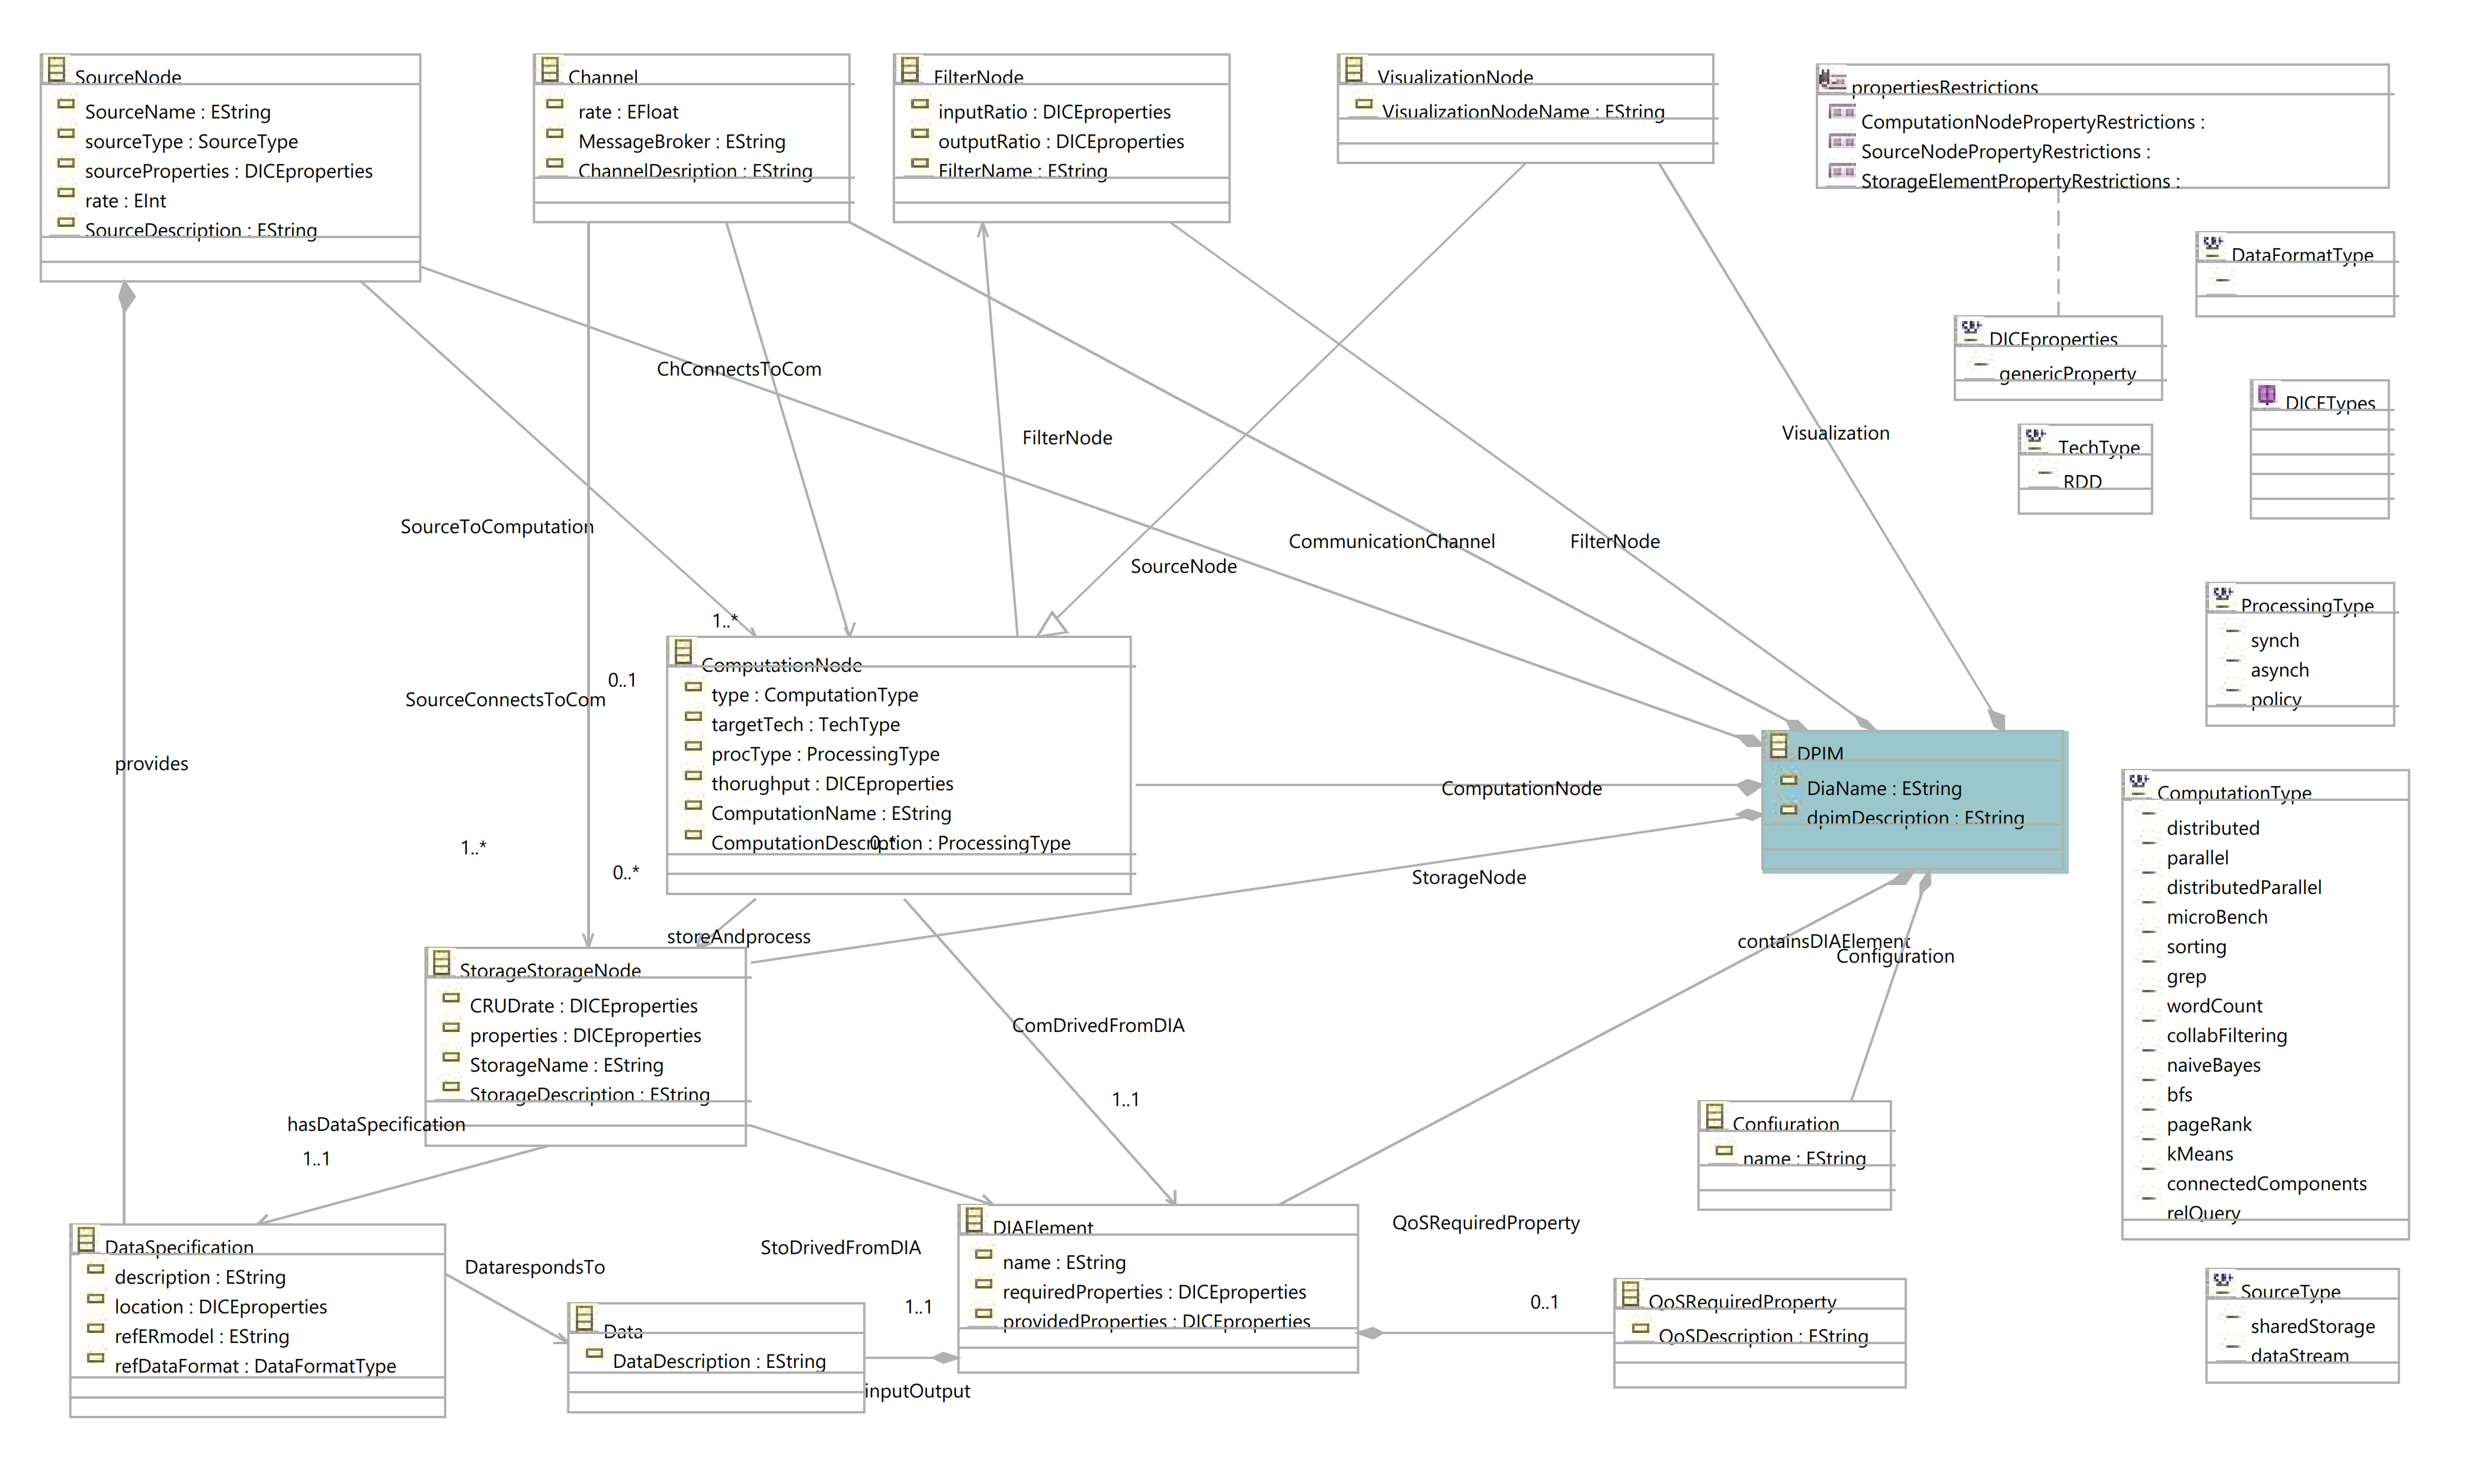
\includegraphics[width=\textwidth]{Images/11.png}
\caption{\label{fig:metamodel}DICE DPIM metamodel.}
\end{sidewaysfigure}

\begin{figure}
\centering
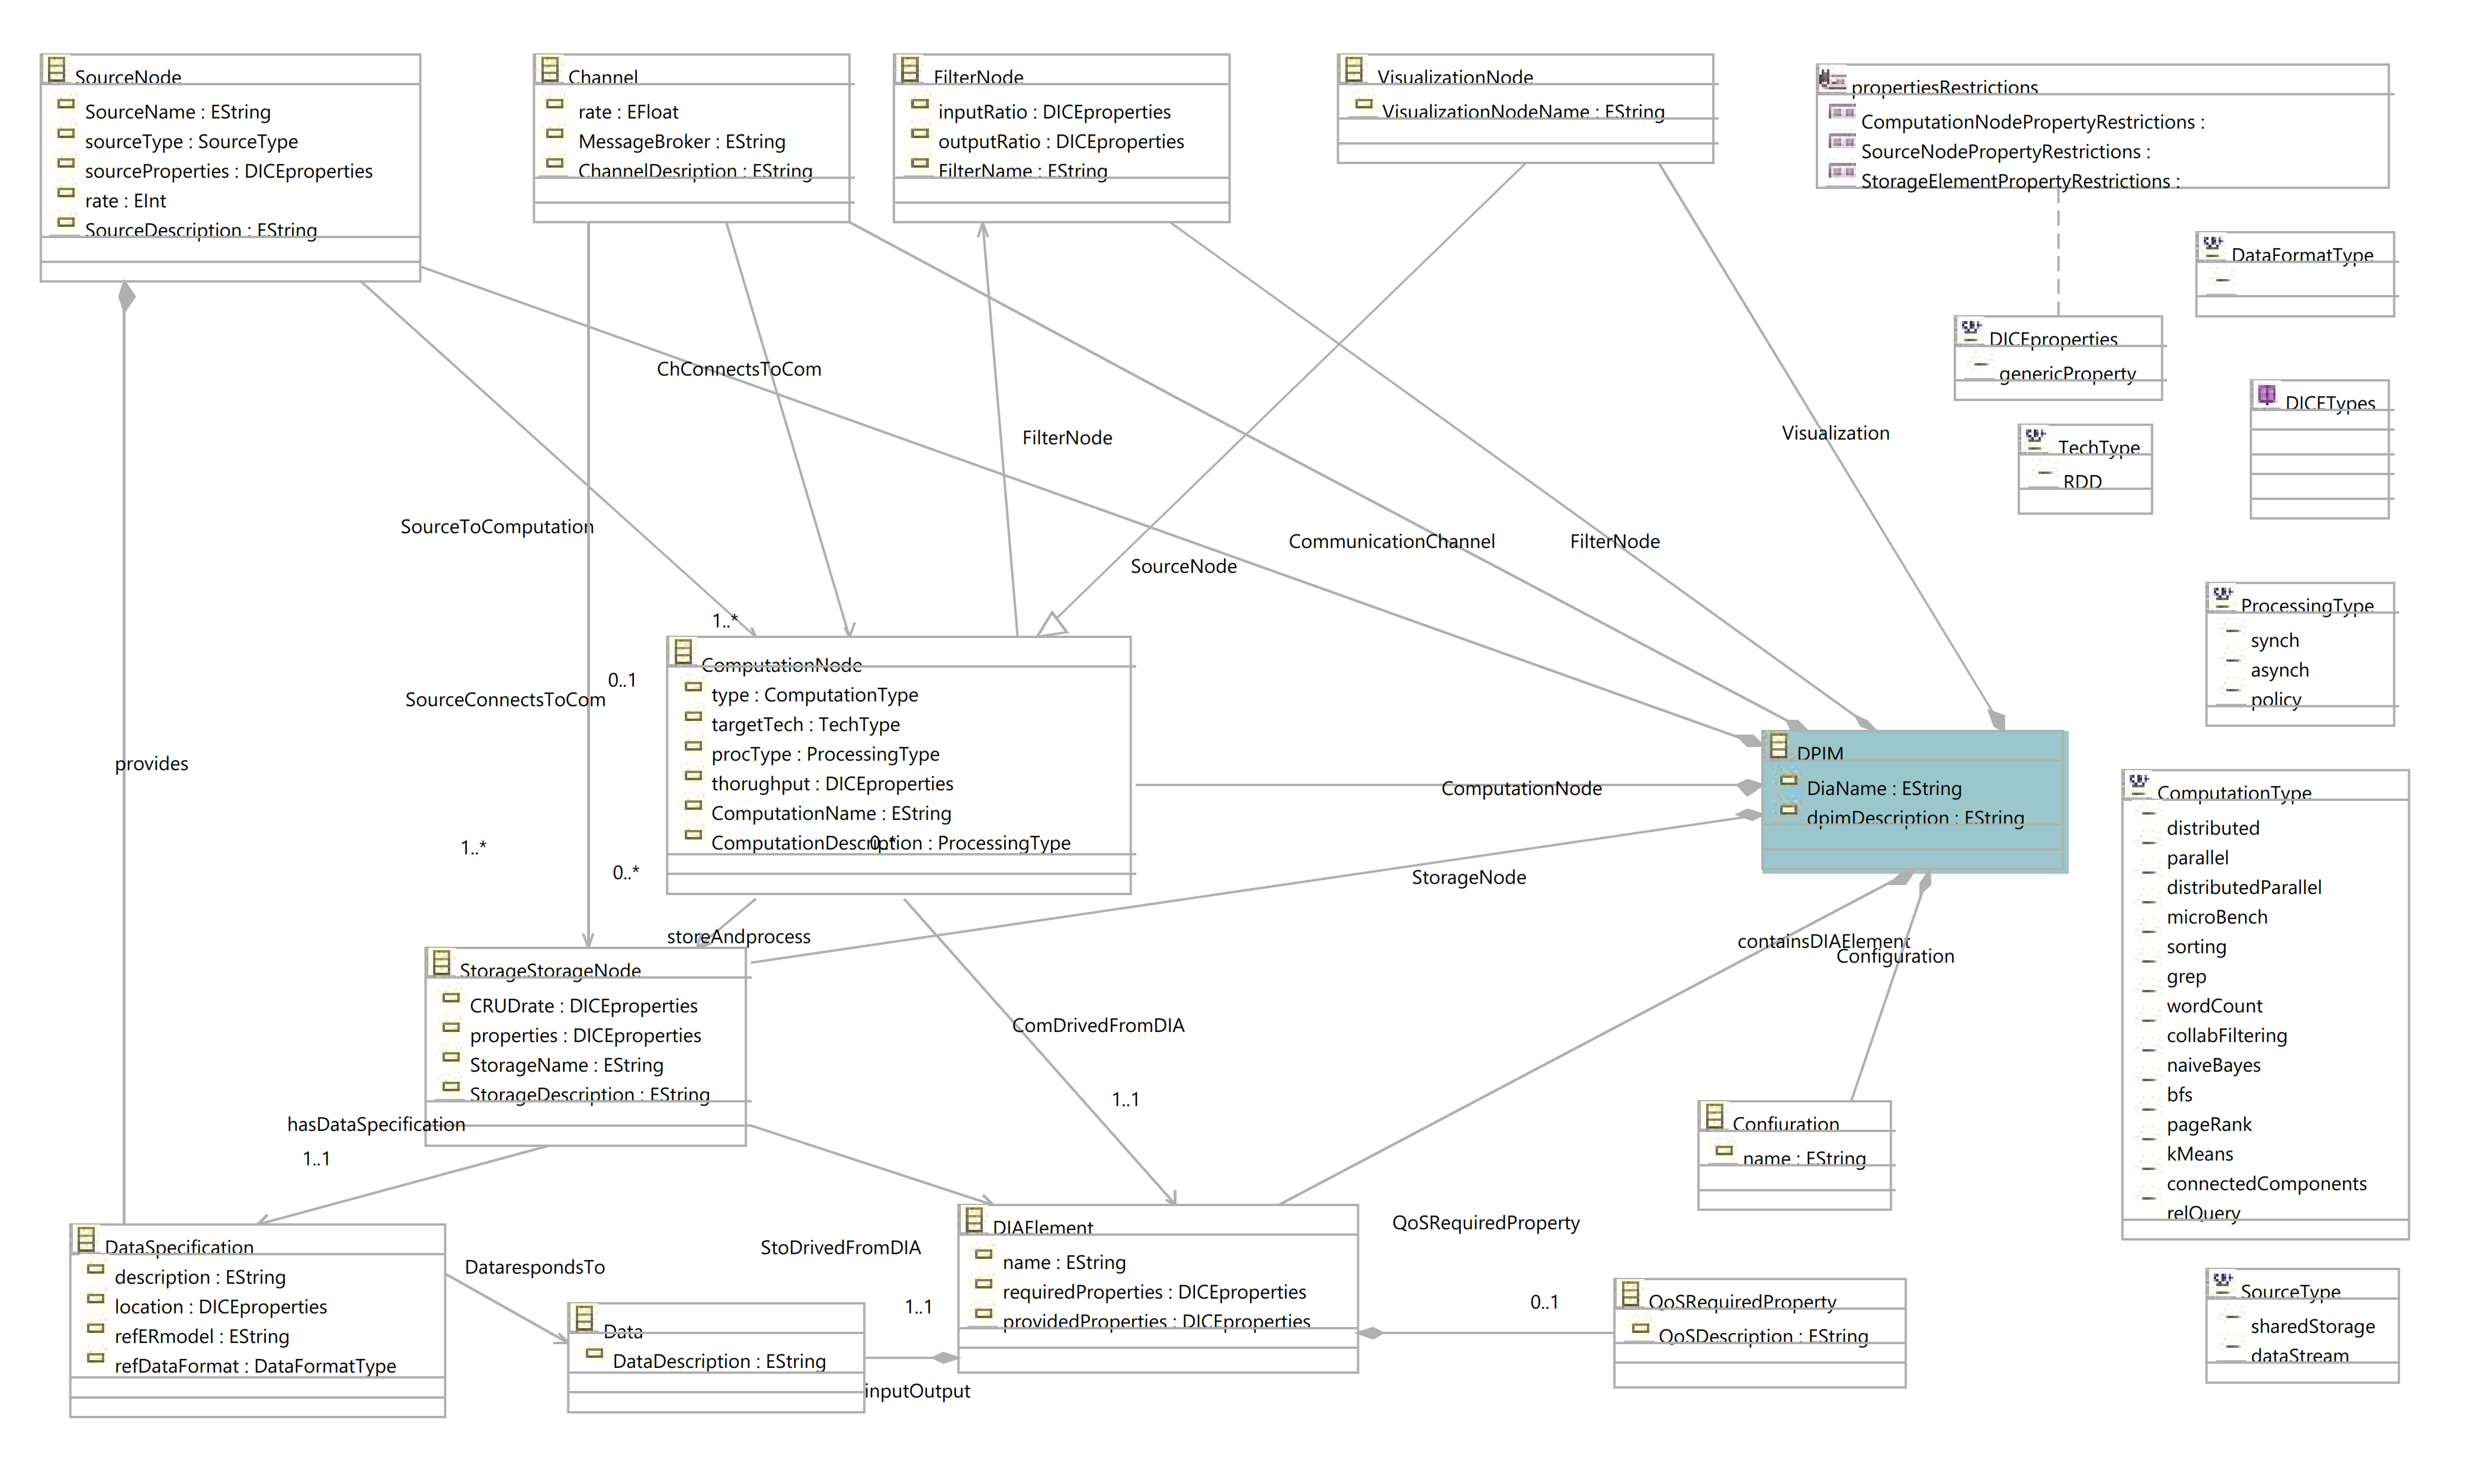
\includegraphics[width=\textwidth]{Images/11.png}
\caption{\label{fig:metamodel2}DICE DPIM metamodel in portrait form.}
\end{figure}

Here is the command to refer to another element (section, figure, table, ...) in the document: \emph{As discussed in Section~\ref{sect:overview} and as shown in Figure~\ref{fig:metamodel}, ...}. Here is how to introduce a bibliographic citation~\cite{DAM}. Bibliographic references should be included in a \texttt{.bib} file. 

Table generation is a bit complicated in Latex. You will soon become proficient, but to start you can rely on tools or external services. See for instance this \href{https://www.tablesgenerator.com}{https://www.tablesgenerator.com}. 

\subsection{Product perspective}
\subsection{Product functions}
the product will be used by farmers, policy makers and agronomists
\subsection{User characteristics}
\subsection{Assumptions, dependencies and constraints}
Assumptions TODO :
\begin{itemize}
	\item
	Cropping seasons are the same on the whole Telengana State and follow the Kharif/Rabi calendar (see Recommended System of Breeder Seed Indent and Supply)
\end{itemize}
\subsubsection{Domain Properties}
here are some domain properties/assumptions
\begin{itemize}
	\item
	DP1 : Every farmer has a smartphone (with geo-tracking,... properties)
	\item
	DP2 : Soil moisture data are updated every 2 days
	\item
	DP : Rainfall conditions are daily updated
	\item
	DP : Rainfall previsions (24/48/72h) are daily updated
	\item
	DP : Data fetched on the different governmental sites are trustworthy reliable
	\item
	DP3 : Farmers are fair when providing data, suggestions and problems
	\item
	DP4 : There are at least 2 farmers and 1 policy maker
	\item
	DP5 : Data from sensors are accurate (in a ... extent)
	\item
	DP6 : Data from the Web are accurate (in a ... extent)
	\item
	DP7 : Sensors are always available, or at least, there is a sufficient number of them to properly describe an area (precision of the DP ?)
	\item
	DP8 : farmers should have received credentials to log in the application
	
\end{itemize}

\subsubsection{use cases}
Here is the diagram for farmers. We suppose they are logged in the application. In case they are not they can simply log in or create an account and then log in.



\begin{table}[htbp]
	\centering
	\begin{tabularx}{\linewidth}{|l|X|}
		\hline
		Name & \multicolumn{1}{c|}{\textit{\textbf{FarmerRegistration}}}                                                   \tabularnewline \hline
		Actors                                               & Farmers                                                    \tabularnewline \hline
		Entry conditions                                              & The farmer is on the DREAM registration form page                                                                                  \tabularnewline \hline
		Event flow                                         & 1.	The system asks for farmer’s data: name, surname, e-mail address, location.                                                                    \tabularnewline 
		& 2.	The farmers fill out the form. The farmer can optionally enable geo-tracking to complete the location field.                                                   \tabularnewline 
		& 3.	The farmer confirms the responses.                                                   \tabularnewline 
		& 4.	The system sends an e-mail containing a validation link to the given e-mail address.                                                \tabularnewline
		& 5.	The system asks the farmer to check his/her e-mail box.                                               \tabularnewline
		& 6.	The farmer clicks on the validation link.                                     \tabularnewline
		& 7.	The system adds the data provided by the farmer to the database.                                  \tabularnewline
		& 8.	Based on the location given by the farmer, the system retrieves the e-mail address of the policy maker dedicated to the farmer newly registered.                               \tabularnewline
		& 9.	The system sends an e-mail to the policy maker to acknowledge that a new farmer has registered.                              \tabularnewline \hline
		Exit conditions & The data are correctly added to the database
		\tabularnewline \hline
		Exceptions & 
		-	The given e-mail address is already in the database. The system displays a message prompting the farmer to modify the dedicated field of the form.  \tabularnewline
		
		&-	The data provided by the farmer have an invalid type or the e-mail address is incorrect. The system displays a message prompting the farmer to modify the dedicated field(s) of the form. 
		\tabularnewline
		&-	There is no registered policy maker dedicated to the area. In that case, no acknowledgement e-mail is sent, but instead a warning message is sent to the developer to urge him/her to contact the adequate policy maker. 
		\tabularnewline
		\hline
	\end{tabularx}   
\end{table}

\begin{table}[htbp]
	\centering
	\begin{tabularx}{\linewidth}{|l|X|}
		\hline
		Name & \multicolumn{1}{c|}{\textit{\textbf{ProductionRelease}}}                                                   \tabularnewline \hline
		Actors                                               & Farmers                                                    \tabularnewline \hline
		Entry conditions                                              & The farmer has begun the cropping season (and eventually finished). \tabularnewline
		&The farmer is already registered on the DREAM platform
		                                                                          \tabularnewline \hline
		Event flow                                         & 1.	The farmer logs in on the platform and clicks on the “Release production data” tab.                                                                   \tabularnewline 
		& 2.	The farmer clicks on the “New release” button                                                   \tabularnewline 
		& 3.	The system displays a form with the following fields: seed variety (to be chosen among a certain list), seed rate, production amount, surface area of the cultivated fields, fertilizer (can be several, to be chosen among a certain list), amount of fertilizer used (one field per fertilizer used), start and end date.                                                 \tabularnewline 
		& 4.	The farmer completes the fields, with respect to the measure units given by the system.                                           \tabularnewline
		& 5.	The farmer confirms.                                               \tabularnewline
		& 6.	The system adds the data to the database.      
		\tabularnewline \hline
		Exit conditions 
		& 
		The data are correctly added to the database
		\tabularnewline \hline
		Exceptions 
		& 
		-	The data provided by the farmer have an invalid type. The system displays a message prompting the farmer to modify the dedicated field(s) of the form
		\tabularnewline
		\hline
	\end{tabularx}   
\end{table}

\begin{table}[htbp]
	\centering
	\begin{tabularx}{\linewidth}{|l|X|}
		\hline
		Name & \multicolumn{1}{c|}{\textit{\textbf{ForumCreation}}}                                                   \tabularnewline \hline
		Actors                                               & Farmers                                                    \tabularnewline \hline
		Entry conditions                                              &
		The farmer is already registered on the DREAM platform
		\tabularnewline
		Event flow                                         & 1.	The farmer logs in on the platform and clicks on the “Forum” tab.                                           \tabularnewline 
		& 2.	The farmer clicks on the “New topic” button.                                            \tabularnewline 
		& 3.	The farmer completes the title and message fields                                            \tabularnewline 
		& 4.	The farmer can optionally add some tags to characterize the topic                                    
		                  \tabularnewline 
		&
		5.	The system adds the topic to the database
		\tabularnewline \hline
		Exit conditions 
		&  The data are correctly added to the database
		\tabularnewline \hline
		Exceptions 
		& 
		-	The data provided by the farmer have an invalid type. The system displays a message prompting the farmer to modify the dedicated field(s) of the form.
		\tabularnewline
		&-	The title or the message is empty. The system displays a message prompting the farmer to fill them both
		
		\tabularnewline
		\hline
	\end{tabularx}   
\end{table}

\begin{table}[htbp]
	\centering
	\begin{tabularx}{\linewidth}{|l|X|}
		\hline
		Name & \multicolumn{1}{c|}{\textit{\textbf{}}}                                                   \tabularnewline \hline
		Actors                                               & Farmers                                                    \tabularnewline \hline
		Entry conditions                                              &
		\tabularnewline
		&
		\tabularnewline \hline
		Event flow                                         &                                            \tabularnewline 
		&                                            \tabularnewline 
		&                                            \tabularnewline 
		&                                     \tabularnewline
		&                                            \tabularnewline
		&                                      \tabularnewline
		&                                 \tabularnewline
		&                               \tabularnewline
		&                               \tabularnewline \hline
		Exit conditions 
		& 
		\tabularnewline \hline
		Exceptions 
		& 
		\tabularnewline
		\hline
	\end{tabularx}   
\end{table}

\begin{figure}
	\centering
	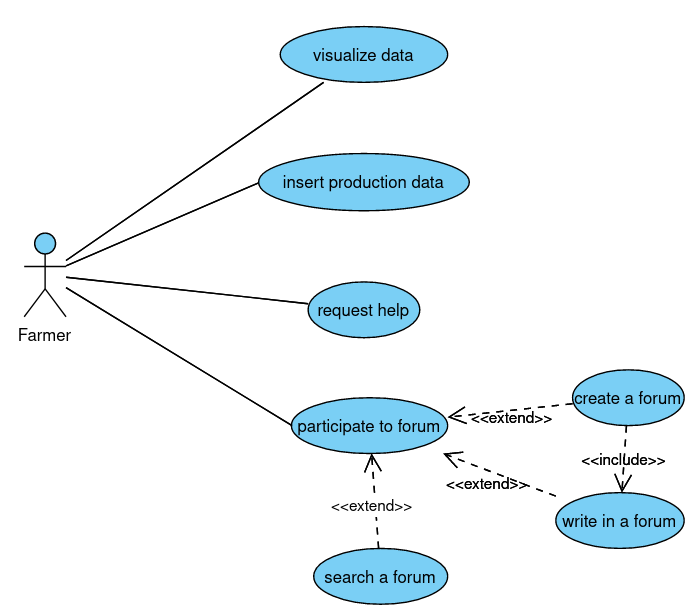
\includegraphics[width=\textwidth]{Images/use-case-farmer.png}
	\caption{\label{fig:usecasefarmer}Use case diagram for logged in farmer}
\end{figure}

\begin{figure}
	\centering
	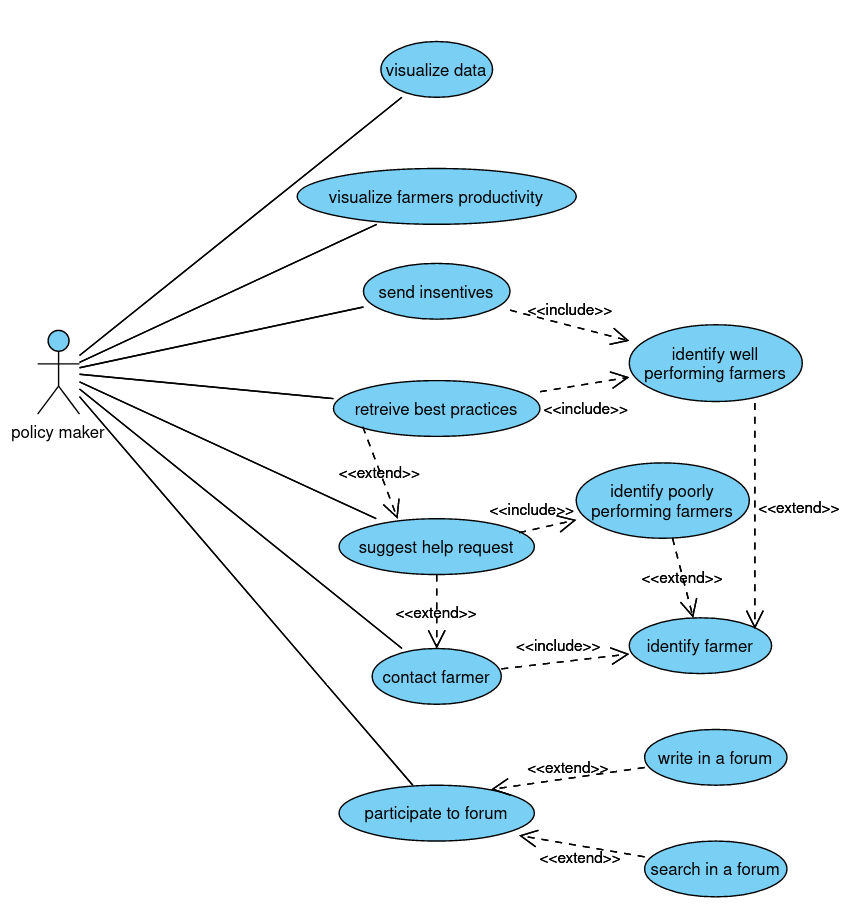
\includegraphics[width=\textwidth]{Images/use-case-policy.png}
	\caption{\label{fig:usecasepolicymakers}Use case diagram for logged in policy makers}
\end{figure}


%------------------------------------------------------------------------------------------------------------------------------------------------
\clearpage
{\color{Blue}{\section{Specific Requirements}}}
\label{sect:requirements}
Organize this section according to the rules defined in the project description. 

\subsection{External Interface Requirements}
\subsubsection{User interfaces}
The user interface will be responsive and should be multiple platform. Even if it should be mainly done for phones. \newline
Where as the application for policy makers should be also responsive but mainly optimized for computer.

First we will present the interfaces for farmers. They are not exhaustive but the goal here is to give a good overview of what the app will look like. The figure \ref{Fig:interface_login} represents the general login page. Depending on the mail the user will then be a farmer or a policy maker.
\begin{figure}[H]
	\centering
	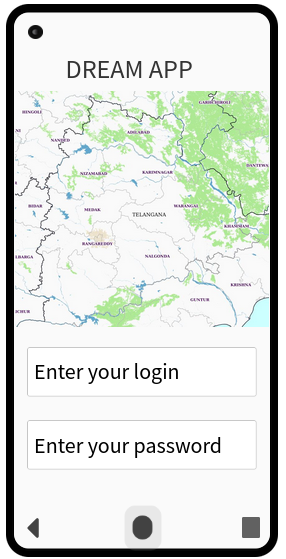
\includegraphics[width=0.2\columnwidth]{Images/login.png}
	\caption{login from a phone}
	\label{Fig:interface_login}
\end{figure}

The figure \ref{Fig:interface_forum} shows the view of the forum on a phone, this view as the others will also be visible from a computer as all the app will be responsive. Next to it the figure \ref{Fig:interface_meteo} gives access to the main data simply and in a rapid way.
\begin{figure}[H]
	\begin{minipage}{0.48\textwidth}
		\centering
		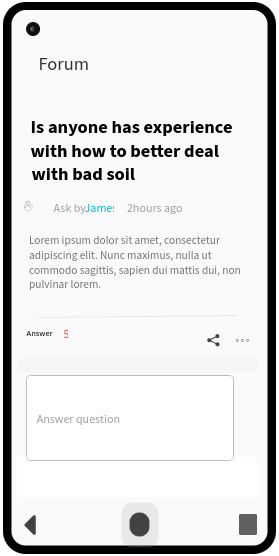
\includegraphics[width=0.6\columnwidth]{Images/forum.png}
		\caption{forum from a phone}
		\label{Fig:interface_forum}
	\end{minipage}
	\begin{minipage}{0.48\textwidth}
		\centering
		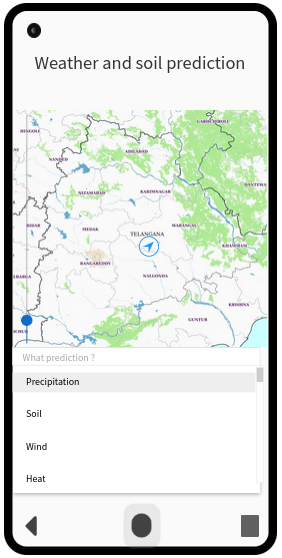
\includegraphics[width=0.6\columnwidth]{Images/meteo.png}
		\caption{have access to data}
		\label{Fig:interface_meteo}
	\end{minipage}\hfill
\end{figure}
\begin{figure}[H]
	\centering
	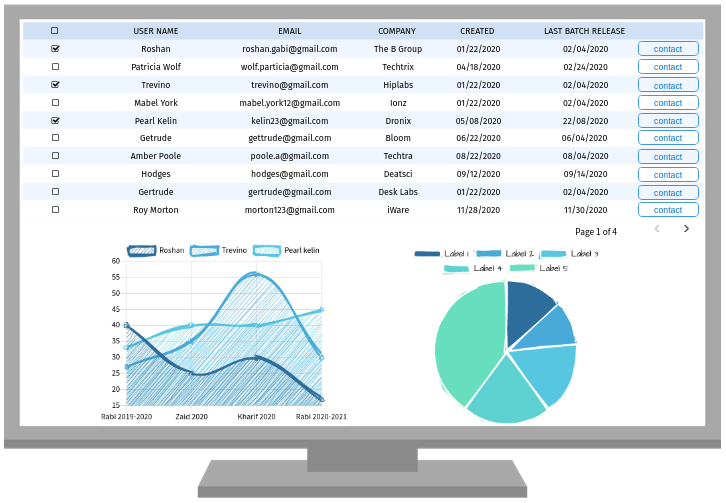
\includegraphics[width=0.8\columnwidth]{Images/visualize_farmers.png}
	\caption{Policy Maker comparing farmer on different factors}
	\label{Fig:interface_visu_farmers}
\end{figure}

\begin{figure}[H]
	\centering
	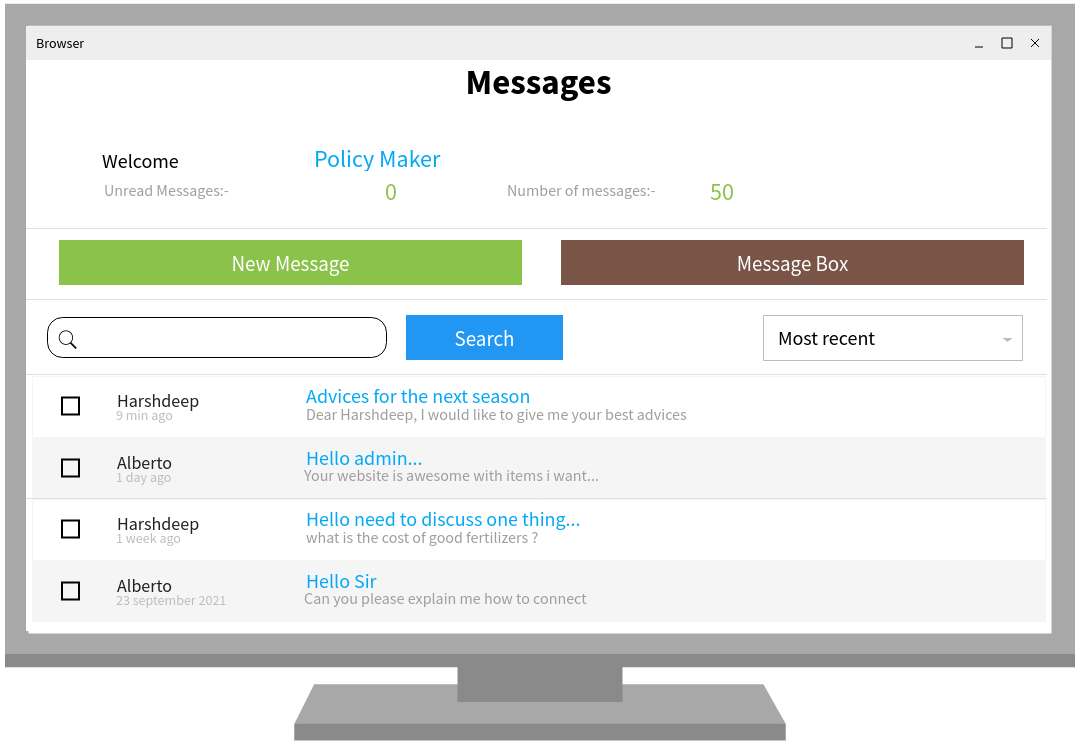
\includegraphics[width=0.8\columnwidth]{Images/messages_policy_maker.png}
	\caption{Policy Maker messages}
	\label{Fig:interface_messages_policy_maker}
\end{figure}
% do not display the following
\iffalse
\subsubsection{Hardware Interfaces}
\subsubsection{Software Interfaces}
\fi % end of will not apear


\subsubsection{Communication Interfaces}
The communication interfaces of the different sensors is external.
\subsection{Functional requirements}
% Definition  of  use  case  diagrams,  use  cases  and  associated sequence/activity diagrams, and mapping on requirements 
\begin{table}[htbp]
	\centering
	\begin{tabularx}{\linewidth}{|l|X|}
		\hline
		Name & \multicolumn{1}{c|}{\textit{\textbf{FarmerRegistration}}}                                                   \tabularnewline \hline
		Actors                                               & Farmers                                                    \tabularnewline \hline
		Entry conditions                                              & The farmer is on the DREAM registration form page                                                                                  \tabularnewline \hline
		Event flow                                         & 1.	The system asks for farmer’s data: name, surname, e-mail address, location.                                                                    \tabularnewline 
		& 2.	The farmers fill out the form. The farmer can optionally enable geo-tracking to complete the location field.                                                   \tabularnewline 
		& 3.	The farmer confirms the responses.                                                   \tabularnewline 
		& 4.	The system sends an e-mail containing a validation link to the given e-mail address.                                                \tabularnewline
		& 5.	The system asks the farmer to check his/her e-mail box.                                               \tabularnewline
		& 6.	The farmer clicks on the validation link.                                     \tabularnewline
		& 7.	The system adds the data provided by the farmer to the database.                                  \tabularnewline
		& 8.	Based on the location given by the farmer, the system retrieves the e-mail address of the policy maker dedicated to the farmer newly registered.                               \tabularnewline
		& 9.	The system sends an e-mail to the policy maker to acknowledge that a new farmer has registered.                              \tabularnewline \hline
		Exit conditions & The data are correctly added to the database
		\tabularnewline \hline
		Exceptions & 
		-	The given e-mail address is already in the database. The system displays a message prompting the farmer to modify the dedicated field of the form.  \tabularnewline
		
		&-	The data provided by the farmer have an invalid type or the e-mail address is incorrect. The system displays a message prompting the farmer to modify the dedicated field(s) of the form. 
		\tabularnewline
		&-	There is no registered policy maker dedicated to the area. In that case, no acknowledgement e-mail is sent, but instead a warning message is sent to the developer to urge him/her to contact the adequate policy maker. 
		\tabularnewline
		\hline
	\end{tabularx}   
\end{table}

\begin{table}[htbp]
	\centering
	\begin{tabularx}{\linewidth}{|l|X|}
		\hline
		Name & \multicolumn{1}{c|}{\textit{\textbf{ProductionRelease}}}                                                   \tabularnewline \hline
		Actors                                               & Farmers                                                    \tabularnewline \hline
		Entry conditions                                              & The farmer has begun the cropping season (and eventually finished). \tabularnewline
		&The farmer is already registered on the DREAM platform
		\tabularnewline \hline
		Event flow                                         & 1.	The farmer logs in on the platform and clicks on the “Release production data” tab.                                                                   \tabularnewline 
		& 2.	The farmer clicks on the “New release” button                                                   \tabularnewline 
		& 3.	The system displays a form with the following fields: seed variety (to be chosen among a certain list), seed rate, production amount, surface area of the cultivated fields, fertilizer (can be several, to be chosen among a certain list), amount of fertilizer used (one field per fertilizer used), start and end date.                                                 \tabularnewline 
		& 4.	The farmer completes the fields, with respect to the measure units given by the system.                                           \tabularnewline
		& 5.	The farmer confirms.                                               \tabularnewline
		& 6.	The system adds the data to the database with the status "Complete".      
		\tabularnewline \hline
		Exit conditions 
		& 
		The data are correctly added to the database
		\tabularnewline \hline
		Exceptions 
		& 
		-	The data provided by the farmer have an invalid type. The system displays a message prompting the farmer to modify the dedicated field(s) of the form
		\tabularnewline
		&-	All the data are not provided (e.g. the end date, the production amount) because cropping has not ended yet. The data are added to the database with an “Incomplete” status. If seed variety, seed rate, surface area or start date are not provided, the system displays an error message
		\tabularnewline
		\hline
	\end{tabularx}   
\end{table}

\begin{table}[htbp]
	\centering
	\begin{tabularx}{\linewidth}{|l|X|}
		\hline
		Name & \multicolumn{1}{c|}{\textit{\textbf{ForumCreation}}}                                                   \tabularnewline \hline
		Actors                                               & Farmers                                                    \tabularnewline \hline
		Entry conditions                                              &
		The farmer is already registered on the DREAM platform
		\tabularnewline
		Event flow                                         & 1.	The farmer logs in on the platform and clicks on the “Forum” tab.                                           \tabularnewline 
		& 2.	The farmer clicks on the “New topic” button.                                            \tabularnewline 
		& 3.	The farmer completes the title and message fields                                            \tabularnewline 
		& 4.	The farmer can optionally add some tags to characterize the topic                                    
		\tabularnewline 
		&
		5.	The system adds the topic to the database
		\tabularnewline \hline
		Exit conditions 
		&  The data are correctly added to the database
		\tabularnewline \hline
		Exceptions 
		& 
		-	The data provided by the farmer have an invalid type. The system displays a message prompting the farmer to modify the dedicated field(s) of the form.
		\tabularnewline
		&-	The title or the message is empty. The system displays a message prompting the farmer to fill them both.
		\tabularnewline
		\hline
	\end{tabularx}   
\end{table}

\begin{table}[htbp]
	\centering
	\begin{tabularx}{\linewidth}{|l|X|}
		\hline
		Name & \multicolumn{1}{c|}{\textit{\textbf{PredictionCheck}}}                                                   \tabularnewline \hline
		Actors                                               & Farmers                                                    \tabularnewline \hline
		Entry conditions                                              &
		The farmer is already registered on the DREAM platform
		\tabularnewline
		&
		\tabularnewline \hline
		Event flow                                         & 1.	The farmer logs in on the platform                                         \tabularnewline 
		& 2.	From the homepage, the farmer clicks on the desired button, between “soil”, “weather” and “vegetation index”.                                          \tabularnewline 
		& 3.	Based on the location of the farmer, the system displays a map for the conditions (and eventually another one for the predictions), with the time period.                                           \tabularnewline 
		& 4.	The farmer can optionally zoom in/out and move on the map provided by the system.                                    \tabularnewline \hline
		Exit conditions 
		& The farmer leaves the homepage
		\tabularnewline \hline
		Exceptions 
		& -	There is no data corresponding to the current time or the location of the farmer. In the first case, the system proposes to display results for a close time (if it exists). In the second case, it zooms out until finding a place where data are available (if they exist)
		\tabularnewline
		\hline
	\end{tabularx}   
\end{table}

\begin{table}[htbp]
	\centering
	\begin{tabularx}{\linewidth}{|l|X|}
		\hline
		Name & \multicolumn{1}{c|}{\textit{\textbf{RequestForProductionData}}}                                                   \tabularnewline \hline
		Actors                                               & Farmers                                                    \tabularnewline \hline
		Entry conditions                                        
		& The farmer is already registered on the DREAM platform and has not confirmed the data for the last cropping season.
		\tabularnewline
		&
		The current date is in a 15 days-range before the end of a cropping season (15/11-01/12, 15/04-01/5 or 15/07-01/08).
		\tabularnewline \hline
		Event flow                                         & 1.	The system sends an e-mail to recall the farmer to release the production data                                           \tabularnewline 
		& 2.	The farmer logs in on the platform.                                             \tabularnewline 
		& 3.	The system displays a notification with a link to the “Release production data” tab.                                           \tabularnewline 
		& 4.	The farmer clicks on the link.                                    \tabularnewline
		& 5.	The system displays the “Release production data” tab, with an additional “Confirm the data for this season” button.                                           \tabularnewline
		& 6.	The farmer eventually creates a new release or completes the releases with an "Incomplete" (see ProductionRelease use case).                                     \tabularnewline
		& 7.	Within 15 days, the farmer clicks on the button “Confirm the data for this season”                                \tabularnewline
		& 8.	The system adds the farmer to the list of farmers who completed their release for the season                              \tabularnewline
		& 9.	The system hides the button “Confirm the data for this season”                       \tabularnewline \hline
		Exit conditions 
		& The system adds the farmer to the list of farmers who completed their release 
		\tabularnewline \hline
		Exceptions 
		& 
		-	The farmer does not click on the button “Confirm the data for this season”. At every log in, the system will display the notification to release the data production
		\tabularnewline
		&
		-	The farmer adds or modifies a production data release after having clicked on the button “Confirm the data for this season”. The system removes the farmer from the list of farmers who completed their release for the season. The system displays the button “Confirm the data for this season” again
		\tabularnewline
		\hline
	\end{tabularx}   
\end{table}

\begin{table}[htbp]
	\centering
	\begin{tabularx}{\linewidth}{|l|X|}
		\hline
		Name & \multicolumn{1}{c|}{\textit{\textbf{TopicResearch}}}                                                   \tabularnewline \hline
		Actors                                               & Farmer, Policy Maker                                                   \tabularnewline \hline
		Entry conditions                                              & The actor is already registered on the DREAM platform
		\tabularnewline
		&
		\tabularnewline \hline
		Event flow                                         & 1.	The actor logs in on the platform and clicks on the “Forum” tab.                                           \tabularnewline 
		& 2.	The actor clicks on the “Search” button.                                           \tabularnewline 
		& 3.	The system displays a search bar and two optional filters: date and tags.                                           \tabularnewline 
		& 4.	The actor completes the field and eventually add some filters.                                    \tabularnewline
		& 5.	The actor confirms the request.                                           \tabularnewline
		& 6.	The system fetches and displays the list of results.                                     \tabularnewline
		& 7.	The actor clicks on one of them.                                \tabularnewline
		& 8.	The system displays the discussion thread on the topic.                              \tabularnewline
		& 9.	The actor can optionally add a message, reply to another one, or put a thumb up/down to someone’s contribution. 
		\tabularnewline
		& 10.	The systems commits the eventual updates in the database                             \tabularnewline \hline
		Exit conditions 
		& The actor leaves the "Forum" tab
		\tabularnewline \hline
		Exceptions 
		& -	The system doesn’t find any result that matches to the actor request. It displays an error message and proposes to make another request.
		\tabularnewline
		& -	The data provided by the actor have an invalid type. The system displays a message prompting  to modify the fields concerned.
		\tabularnewline
		\hline
	\end{tabularx}   
\end{table}


\begin{table}[htbp]
	\centering
	\begin{tabularx}{\linewidth}{|l|X|}
		\hline
		Name & \multicolumn{1}{c|}{\textit{\textbf{ContactingPoorlyPerformingFarmers}}}                                                   \tabularnewline \hline
		Actors                                               & Policy Maker                                                    \tabularnewline \hline
		Entry conditions                                              &
		The policy maker is already registered on the DREAM platform.
		The farmers have already released their production data.
		\tabularnewline
		&
		\tabularnewline \hline
		Event flow                                         & 1.	The policy maker logs in on the platform and clicks on the “Visualize productivity” tab.                                         \tabularnewline 
		& 2.	The policy maker chooses a metric, a period, ticks the “bottom” box and enters the number of results wanted.                                           \tabularnewline 
		& 3.	The system fetches and displays the results ordered by the performance metric.                                           \tabularnewline 
		& 4.	The policy maker clicks on some farmers line.                                    \tabularnewline
		& 5.	The system displays more precise information about the results (seed variety and rate, field surface, production amount, fertilizers, amount of fertilizer used, start and end date).                                           \tabularnewline
		& 6.	The policy maker clicks on the “Contact” button.                                     \tabularnewline
		& 7.	The policy maker enters a message in the dedicated field and ticks the “help suggestion” box.                                \tabularnewline
		& 8.	The system sends the message to the farmer. The message includes an help request form.                               \tabularnewline \hline
		Exit conditions 
		& The message arrives in the farmer’s personal contact tab
		\tabularnewline \hline
		Exceptions 
		& -	There is not any result on the policy maker request (because no production data release or lacking some fields for the chosen metric). The system displays an error message and eventually proposes to choose another metric.
		\tabularnewline
		\hline
	\end{tabularx}   
\end{table}

\begin{table}[htbp]
	\centering
	\begin{tabularx}{\linewidth}{|l|X|}
		\hline
		Name & \multicolumn{1}{c|}{\textit{\textbf{HelpRequest}}}                                                   \tabularnewline \hline
		Actors                                               & Farmer                                               \tabularnewline \hline
		Entry conditions                                              &
		The farmer is already registered on the DREAM platform.
		\tabularnewline
		&
		\tabularnewline \hline
		Event flow                                         & 1.	The policy maker logs in on the platform and clicks on the “Contact” tab.                                        \tabularnewline 
		& 2.	The farmer clicks on the “New help request” button.                                   \tabularnewline 
		& 3.	The farmer writes down a message and ticks for the correct level of priority.                                           \tabularnewline 
		& 4.	The farmer confirms.                                   \tabularnewline
		& 5.	The system sends the message to the dedicated policy maker’s messages tab.                                          \tabularnewline
		& 6.	An e-mail is sent to the policy maker’s address                                    \tabularnewline
		\hline
		Exit conditions 
		& The message arrives in the policy maker’s personal box
		\tabularnewline \hline
		Exceptions 
		& 
		-	There is no registered policy maker dedicated to the area. In that case, an error message is displayed to the farmer, and a warning message is sent to the developer to urge him/her to contact the adequate policy maker.
		\tabularnewline
		\hline
	\end{tabularx}   
\end{table}

\begin{table}[htbp]
	\centering
	\begin{tabularx}{\linewidth}{|l|X|}
		\hline
		Name & \multicolumn{1}{c|}{\textit{\textbf{ContactingWellPerformingFarmers}}}                                                   \tabularnewline \hline
		Actors                                               & Policy Maker                                               \tabularnewline \hline
		Entry conditions                                              &
		The policy maker is already registered on the DREAM platform.
		The farmers have already released their production data.
		\tabularnewline
		&
		\tabularnewline \hline
		Event flow                                         & 1.	The policy maker logs in on the platform and clicks on the “Visualize productivity” tab.                                        \tabularnewline 
		& 2.	The policy maker chooses a metric, a period, ticks the “bottom” box and enters the number of results wanted.                                    \tabularnewline 
		& 3.	The system fetches and displays the results ordered by the performance metric.                                          \tabularnewline 
		& 4.	The policy maker clicks on some farmers line.                                    \tabularnewline
		& 5.	The system displays more precise information about the results (seed variety and rate, field surface, production amount, fertilizers, amount of fertilizer used, start and end date).                                          \tabularnewline
		& 6.	The policy maker clicks on the “Contact” button.                                    \tabularnewline
		& 7.	The policy maker enters a message in the dedicated field and ticks the “e-voucher” box and enters the amount of the incentive. Within the message, the policy maker asks for suggestions to the farmer.                               \tabularnewline
		& 8.	The system sends the message and an e-voucher link to the farmer
		\tabularnewline \hline
		Exit conditions 
		& The message arrives in the farmer’s personal contact tab
		\tabularnewline \hline
		Exceptions 
		& -	There is not any result on the policy maker request (because no production data release or lacking some fields for the chosen metric). The system displays an error message and eventually proposes to choose another metric.
		\tabularnewline
		\hline
	\end{tabularx}   
\end{table}


\begin{figure}
	\centering
	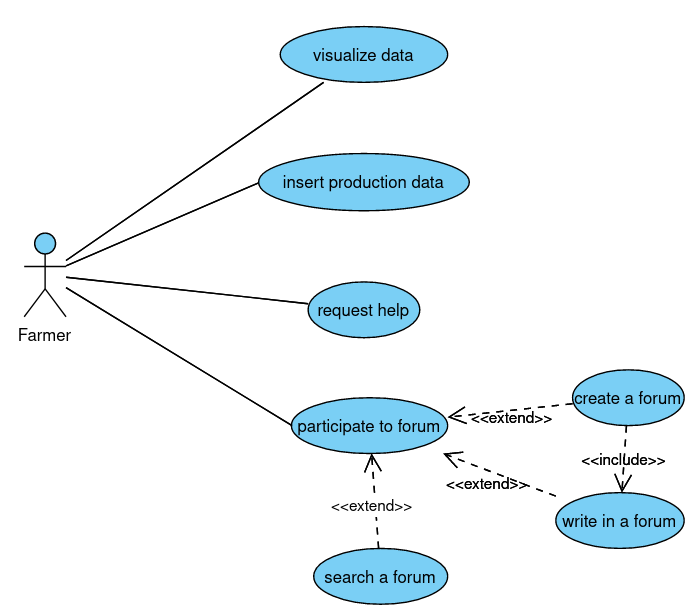
\includegraphics[width=\textwidth]{Images/use-case-farmer.png}
	\caption{\label{fig:usecasefarmer}Use case diagram for logged in farmer}
\end{figure}

\begin{figure}
	\centering
	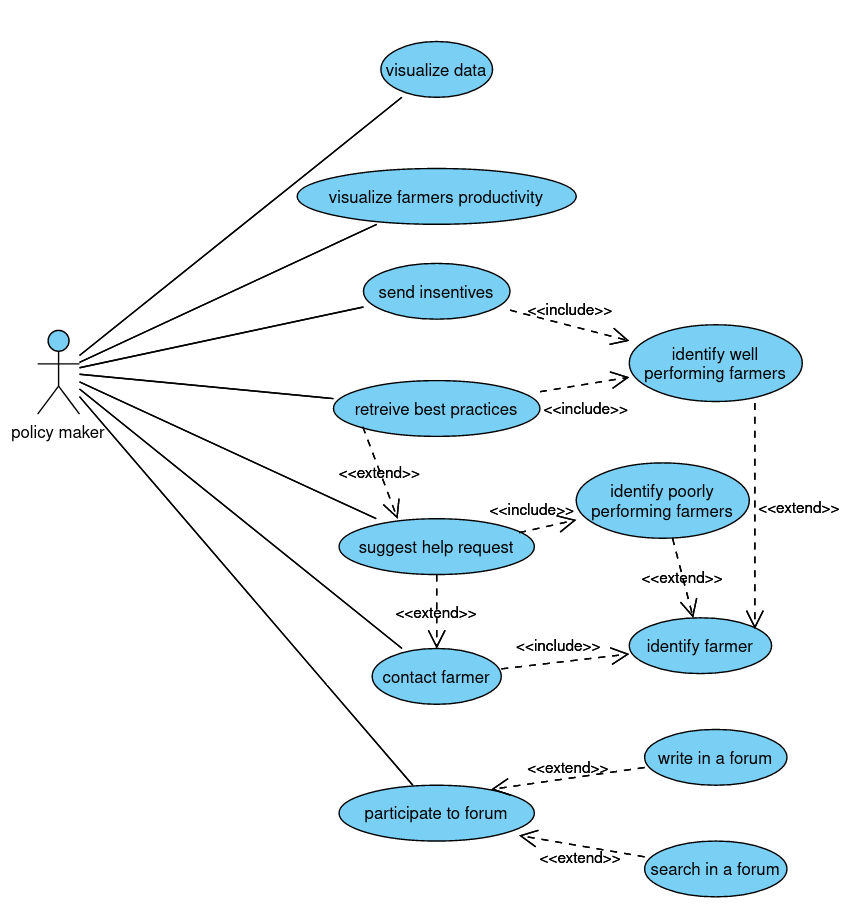
\includegraphics[width=\textwidth]{Images/use-case-policy.png}
	\caption{\label{fig:usecasepolicymakers}Use case diagram for logged in policy makers}
\end{figure}


\begin{figure}
	\centering
	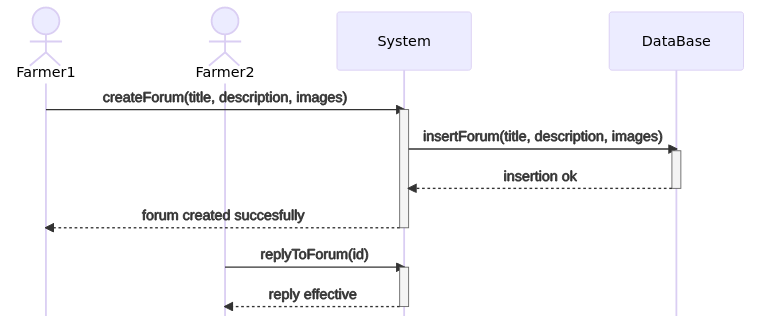
\includegraphics[width=\textwidth]{Images/seq_creation_forum.png}
	\caption{\label{fig:seqcreationforum} Sequence diagram on the creation of a forum and the reply by another farmer}
\end{figure}

\begin{figure}
	\centering
	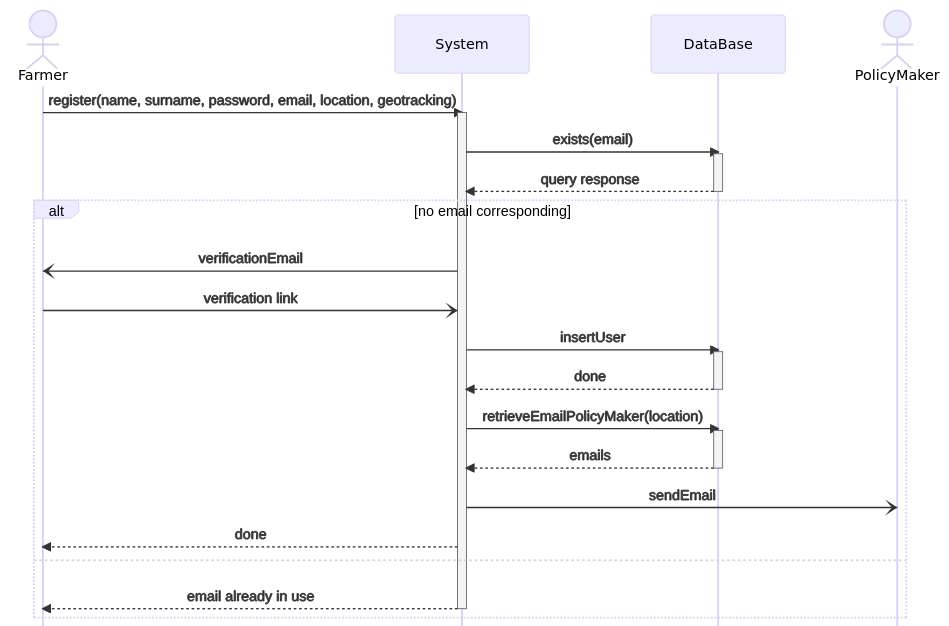
\includegraphics[width=\textwidth]{Images/seq_registration.png}
	\caption{\label{fig:seqregistration} Sequence diagram on the registration of a farmer}
\end{figure}

\begin{figure}
	\centering
	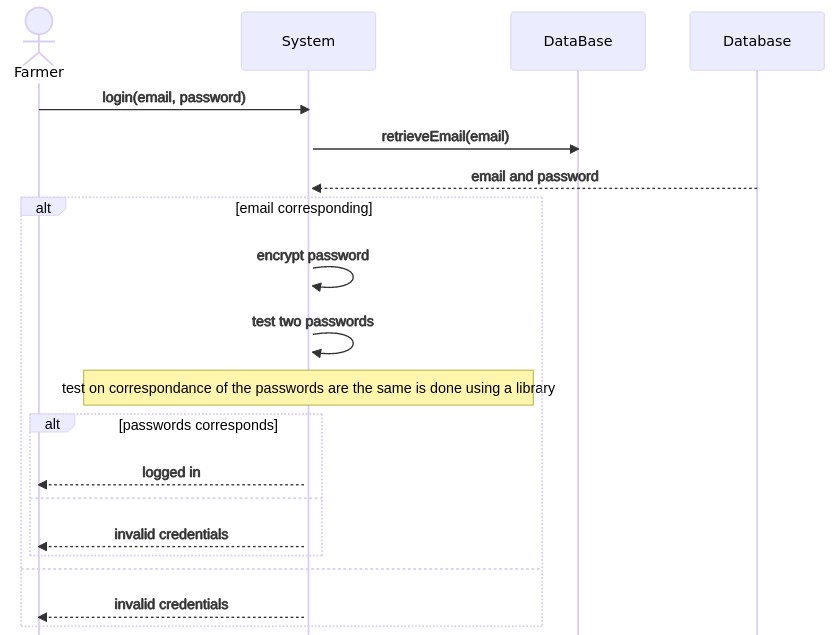
\includegraphics[width=\textwidth]{Images/seq_login.png}
	\caption{\label{fig:seqlogin} Sequence diagram on the login of a farmer}
\end{figure}

\begin{figure}
	\centering
	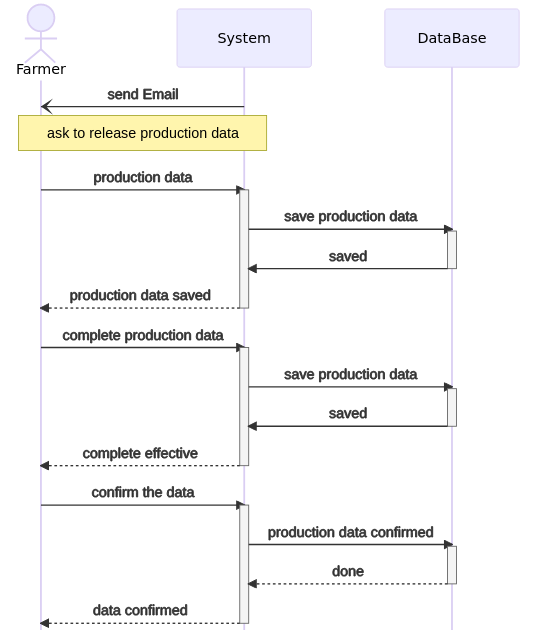
\includegraphics[width=\textwidth]{Images/seq_request_data.png}
	\caption{\label{fig:seqrequestdata} Sequence diagram on the request for production data from a farmer point of view}
\end{figure}

\begin{figure}
	\centering
	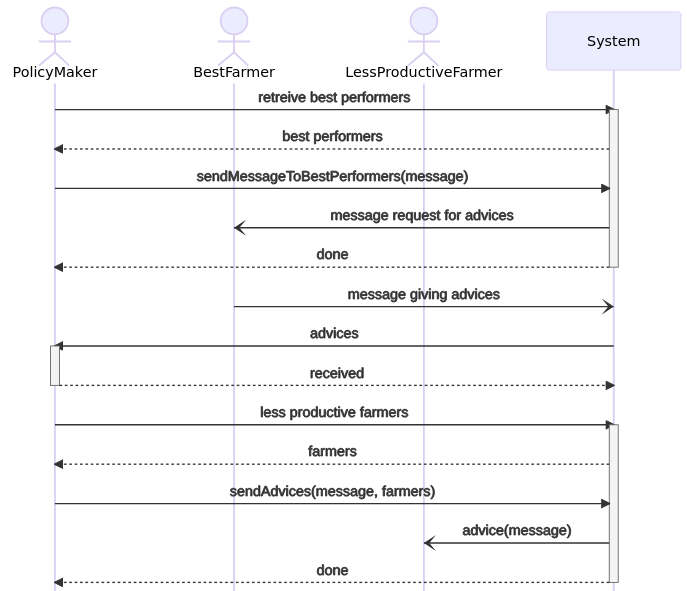
\includegraphics[width=\textwidth]{Images/seq-policy-farmers.png}
	\caption{\label{fig:seq} Sequence diagram showing a policy marker reaching out best performing farmers for advises and send them to less productive farmer}
\end{figure}

\subsection{Performance Requirements}

\subsection{Design Constraints}
\subsubsection{Standards compliance}
\subsubsection{Hardware limitations}
\subsubsection{Any other constraint ??}
Do we keep it ?
\subsection{Software System Attributes}
\subsubsection{Reliability}
\subsubsection{Availability}
\subsubsection{Security}
\subsubsection{Maintainability}
\subsubsection{Portability}


%------------------------------------------------------------------------------------------------------------------------------------------------
\clearpage
{\color{Blue}{\section{Formal Analysis Using Alloy}}}
\label{sect:alloy}
Our Alloy analysis focuses on the production data release and analysis and what they involve. The main goals of the model are the following : 
\begin{itemize}[label=\textbullet]
	\item Define correct rules for (in)complete productions releases and (not) confirmed batches, so that the list of farmers with "confirmed"status is up-to-date.
	\item Define rules to get this list of farmers full at the end of the croping season.
	\item Define rules to provide help to every farmer who performed badly during the previous season.
\end{itemize}

\lstinputlisting[language=alloy]{dream.als}

\begin{figure} [!h]
	\centering
	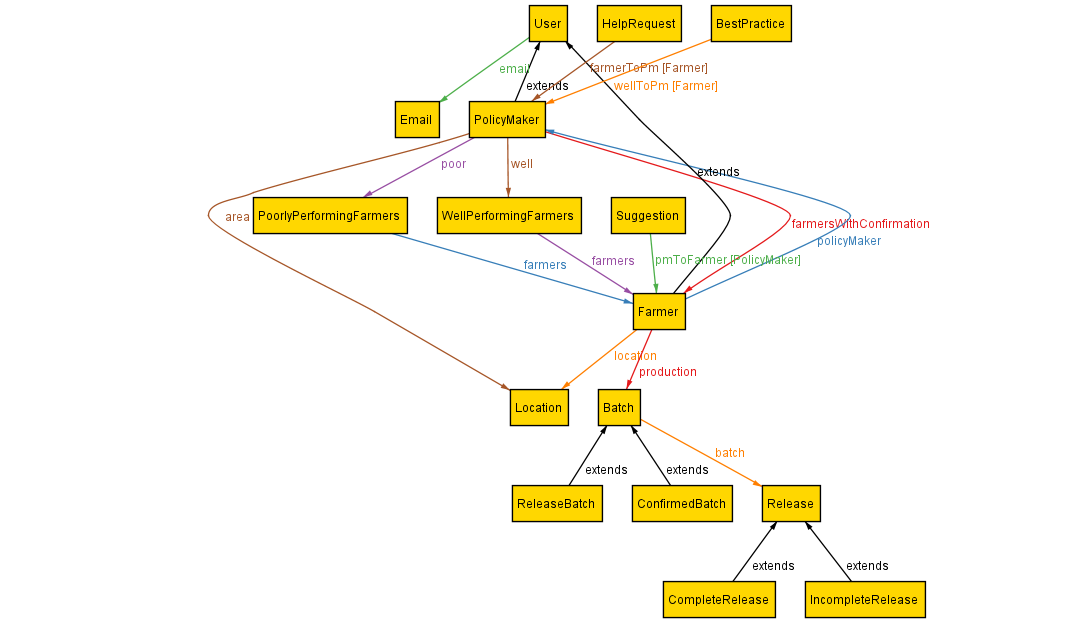
\includegraphics[width=\textwidth]{Images/alloy-metamodel.png}
	\caption{\label{fig:seq} Meta Model}
\end{figure}

%------------------------------------------------------------------------------------------------------------------------------------------------
\clearpage
{\color{Blue}{\section{Effort Spent}}}
\label{sect:effort}
We had a reunion every week on Wednesday morning. 
\subsection{Baudouin De Parcevaux}
\begin{tabular}{| c | c | }
	task & time spent \\
	introduction & 5 \\
 	scope & h\\
 	phenomenas & \\
	scenarios & h\\
 	requirements & h\\
	use cases & h\\
	diagrams & h\\
	Alloy & h\\
	RASD & h\\
\end{tabular}

\subsection{Glen Pouliquen}



%------------------------------------------------------------------------------------------------------------------------------------------------
\clearpage
\addcontentsline{toc}{section}{References}
\bibliographystyle{plain}
\bibliography{main}
%------------------------------------------------------------------------------------------------------------------------------------------------




\end{document}
